\section{Point Cloud Compression}
\label{sec:compression}

\subsection{Rate-Distortion Theory}
\label{ssec:rate-distortion}

Lossy compression is governed by the rate-distortion
function~\cite{shannon1959coding} $R(D)$: the minimum number of bits per
symbol required to represent a source with expected distortion at most $D$.
For a Gaussian source with quadratic distortion,
$R(D) = \frac{1}{2}\log_2(\sigma^2/D)$ bits per sample.
More generally, $R(D)$ is a non-increasing convex function of $D$:
lower distortion always requires higher rate.

\paragraph{Operational rate-distortion.}
A practical compression system cannot achieve the Shannon bound exactly;
it operates at some point $(R, D)$ on or above the theoretical curve.
Modern learned codecs optimise a Lagrangian:
\begin{equation}
  \mathcal{L} = \mathbb{E}\left[d(\mathbf{x}, \hat{\mathbf{x}})\right]
              + \lambda \cdot \mathbb{E}\left[-\log_2 p(\hat{\mathbf{y}})\right],
  \label{eq:rd-lagrangian}
\end{equation}
where the first term is the reconstruction distortion, the second is the
expected rate (cross-entropy under the entropy model), and $\lambda > 0$
controls the rate-distortion tradeoff.
Training a family of models at different $\lambda$ values traces out a
rate-distortion curve.
Lower $\lambda$ prioritises quality (high rate); higher $\lambda$ prioritises
compactness (high distortion).

\paragraph{Entropy coding.}
Given a probability model $p(\hat{\mathbf{y}})$, arithmetic coding achieves
a code length arbitrarily close to the Shannon entropy $-\sum_y p(y)\log_2 p(y)$.
In learned codecs, the entropy model is itself a neural network, trained
jointly with the encoder and decoder to minimise the bound in
Equation~\ref{eq:rd-lagrangian}.

\begin{figure}[t]
\centering
\begin{tikzpicture}[>=Stealth]
  % Plot region: 5.8cm wide, 3.8cm tall
  \def\W{5.8}
  \def\H{3.8}

  % Subtle background and border
  \fill[gray!4] (0,0) rectangle (\W,\H);
  \draw[gray!30] (0,0) rectangle (\W,\H);

  % Light horizontal grid lines
  \foreach \y in {0.95, 1.90, 2.85}
    \draw[gray!18] (0,\y) -- (\W,\y);

  % R-D curve: high quality at low rate, sweeping to high compression
  % Points carefully chosen to be on the curve interior, not clipped
  \draw[blue!65, very thick, smooth]
    plot[tension=0.45] coordinates {
      (0.30,3.50) (0.80,2.90) (1.50,2.25) (2.40,1.70)
      (3.40,1.28) (4.30,0.98) (5.30,0.72)
    }
    node[right, font=\small, blue!70] {$R(D)$};

  % Operating points
  \fill[red!60] (0.80, 2.90) circle (3.5pt);
  \fill[red!60] (2.40, 1.70) circle (3.5pt);
  \fill[red!60] (4.30, 0.98) circle (3.5pt);

  \node[font=\scriptsize, above right=-1pt] at (0.80, 2.90) {$\lambda_1$};
  \node[font=\scriptsize, above right=-1pt] at (2.40, 1.70) {$\lambda_2$};
  \node[font=\scriptsize, above right=-1pt] at (4.30, 0.98) {$\lambda_3$};

  % Annotation: direction of increasing lambda
  \draw[->, gray!50] (0.80, -0.52) -- (4.30, -0.52);
  \node[font=\tiny, gray!60] at (2.55, -0.72) {increasing $\lambda$ (more compression)};

  % Axes
  \draw[->] (0,0) -- (\W+0.40, 0) node[right, font=\small] {Rate (bpp)};
  \draw[->] (0,0) -- (0, \H+0.30) node[above, font=\small] {Quality (PSNR)};
\end{tikzpicture}
\caption{%
  Rate-distortion curve schematic.
  Training a codec at different Lagrange multipliers $\lambda$ traces
  different operating points on the rate-distortion curve: lower $\lambda$
  emphasises distortion reduction (high quality, high rate); higher $\lambda$
  emphasises bit savings (low quality, low rate).
  The curve represents the theoretical achievable boundary; practical
  systems operate on or above it.
}
\label{fig:rd-curve-concept}
\end{figure}

\subsection{Traditional Geometry Codecs}

\paragraph{G-PCC (Geometry-based Point Cloud Compression)~\cite{graziosi2020gpcc}.}
G-PCC is the MPEG geometry codec standard (ISO/IEC 23090-9).
It encodes geometry via recursive octree decomposition: the bounding box
is halved in each dimension until each leaf node contains at most one point.
At each octree level, the occupancy of the eight child nodes is represented
as an 8-bit symbol and arithmetic-coded using a probability model that
conditions on the parent and sibling context.

An alternative \emph{Trisoup} mode approximates the surface within each
leaf node by a planar triangle, enabling efficient coding of smooth surfaces
at low rates where fine voxel detail would be costly.

G-PCC does not introduce spatial bias: its artifacts manifest as
approximately uniform quantisation noise across the surface, independent
of local surface geometry.
This is the key qualitative difference from learned codecs, exploited in
the comparison in Chapter~\ref{ch:oversmoothing}.

\begin{figure}[t]
\centering
% Oblique-projection 3D octree (1.25× scale): x→right, y→upper-right, z→up
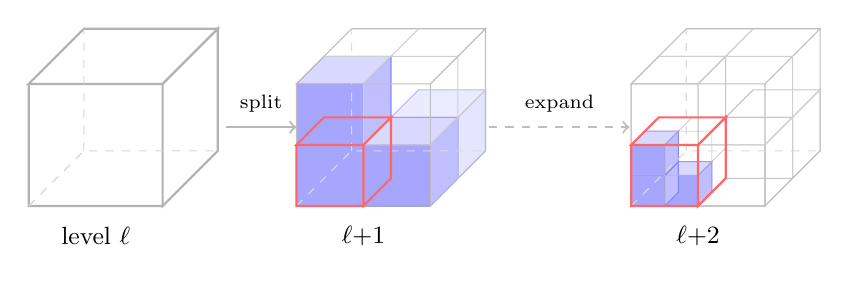
\begin{tikzpicture}[
  x={(0.85cm,0cm)}, y={(0.35cm,0.35cm)}, z={(0cm,0.775cm)},
  font=\small
]

% ── Panel 1: level-ℓ bounding box (outline only) ───────────────
\draw[gray!60, thick]
  (0,0,0)--(2,0,0)--(2,0,2)--(0,0,2)--cycle
  (2,0,0)--(2,2,0)--(2,2,2)--(2,0,2)--cycle
  (0,0,2)--(2,0,2)--(2,2,2)--(0,2,2)--cycle;
\draw[gray!32, dashed]
  (0,0,0)--(0,2,0)--(2,2,0)  (0,2,0)--(0,2,2);
\node[font=\small] at (0.85cm,-0.38cm) {level $\ell$};

% ── Arrow 1 ─────────────────────────────────────────────────────
\draw[->, thick, gray!55] (2.50cm,1.00cm)--(3.40cm,1.00cm);
\node[font=\scriptsize, above] at (2.95cm,1.06cm) {split};

% ── Panel 2: level-(ℓ+1), 4 occupied octants (painter order) ───
% Cube at (5,1,0) [back, draw first]
\fill[blue!15,draw=blue!38,thin]
  (5,1,0)--(6,1,0)--(6,1,1)--(5,1,1)--cycle;   % front
\fill[blue!10,draw=blue!32,thin]
  (6,1,0)--(6,2,0)--(6,2,1)--(6,1,1)--cycle;   % right
\fill[blue!8, draw=blue!28,thin]
  (5,1,1)--(6,1,1)--(6,2,1)--(5,2,1)--cycle;   % top
% Cube at (4,0,0)
\fill[blue!35,draw=blue!55,thin]
  (4,0,0)--(5,0,0)--(5,0,1)--(4,0,1)--cycle;   % front
\fill[blue!25,draw=blue!48,thin]
  (5,0,0)--(5,1,0)--(5,1,1)--(5,0,1)--cycle;   % right
\fill[blue!15,draw=blue!40,thin]
  (4,0,1)--(5,0,1)--(5,1,1)--(4,1,1)--cycle;   % top
% Cube at (5,0,0)
\fill[blue!35,draw=blue!55,thin]
  (5,0,0)--(6,0,0)--(6,0,1)--(5,0,1)--cycle;   % front
\fill[blue!25,draw=blue!48,thin]
  (6,0,0)--(6,1,0)--(6,1,1)--(6,0,1)--cycle;   % right
\fill[blue!15,draw=blue!40,thin]
  (5,0,1)--(6,0,1)--(6,1,1)--(5,1,1)--cycle;   % top
% Cube at (4,0,1) [top-front, last]
\fill[blue!35,draw=blue!55,thin]
  (4,0,1)--(5,0,1)--(5,0,2)--(4,0,2)--cycle;   % front
\fill[blue!25,draw=blue!48,thin]
  (5,0,1)--(5,1,1)--(5,1,2)--(5,0,2)--cycle;   % right
\fill[blue!15,draw=blue!40,thin]
  (4,0,2)--(5,0,2)--(5,1,2)--(4,1,2)--cycle;   % top
% Outer box
\draw[gray!50,thin]
  (4,0,0)--(6,0,0)--(6,0,2)--(4,0,2)--cycle
  (6,0,0)--(6,2,0)--(6,2,2)--(6,0,2)--cycle
  (4,0,2)--(6,0,2)--(6,2,2)--(4,2,2)--cycle;
\draw[gray!28,dashed]
  (4,0,0)--(4,2,0)--(6,2,0)  (4,2,0)--(4,2,2);
\draw[gray!38,thin]
  (5,0,0)--(5,0,2)   (5,0,2)--(5,2,2)
  (4,0,1)--(6,0,1)   (6,0,1)--(6,2,1)
  (6,1,0)--(6,1,2)   (4,1,2)--(6,1,2);
% Highlight the octant being expanded (front-bottom-left)
\draw[red!60, thick]
  (4,0,0)--(5,0,0)--(5,0,1)--(4,0,1)--cycle
  (5,0,0)--(5,1,0)--(5,1,1)--(5,0,1)--cycle
  (4,0,1)--(5,0,1)--(5,1,1)--(4,1,1)--cycle;
\node[font=\small] at (4.25cm,-0.38cm) {$\ell{+}1$};

% ── Arrow 2: Panel 2 right = 5.80cm; Panel 3 left = 7.65cm ─────
\draw[->, thick, gray!50, dashed] (5.84cm,1.00cm)--(7.63cm,1.00cm);
\node[font=\scriptsize, above] at (6.74cm,1.06cm) {expand};

% ── Panel 3: level-(ℓ+2), same 2×2×2 size as Panel 2 ──────────
% Red octant (9,0,0)-(10,1,1) shown subdivided in context.
% Surrounding 3 octants: outline only (ℓ+1 context, not ℓ+2 content).
% Sub-octants (0.5-unit) inside red octant: LR-Bot, LL-Bot, LL-Top.
% Painter order: back outline → bottom sub-octants → right outline
%                → top sub-octant → top outline → box/grid → red border

% Back octant (10,1,0): outline only
\draw[gray!45,thin]
  (10,1,0)--(11,1,0)--(11,1,1)--(10,1,1)--cycle
  (11,1,0)--(11,2,0)--(11,2,1)--(11,1,1)--cycle
  (10,1,1)--(11,1,1)--(11,2,1)--(10,2,1)--cycle;

% LR-Bot sub-octant (9.5,0,0)-(10,0.5,0.5): draw before front-right cube
\fill[blue!35,draw=blue!55,thin]
  (9.5,0,0)--(10,0,0)--(10,0,0.5)--(9.5,0,0.5)--cycle;   % front
\fill[blue!25,draw=blue!48,thin]
  (10,0,0)--(10,0.5,0)--(10,0.5,0.5)--(10,0,0.5)--cycle;   % right
\fill[blue!15,draw=blue!40,thin]
  (9.5,0,0.5)--(10,0,0.5)--(10,0.5,0.5)--(9.5,0.5,0.5)--cycle;   % top

% LL-Bot sub-octant (9,0,0)-(9.5,0.5,0.5)
\fill[blue!35,draw=blue!55,thin]
  (9,0,0)--(9.5,0,0)--(9.5,0,0.5)--(9,0,0.5)--cycle;     % front
\fill[blue!25,draw=blue!48,thin]
  (9.5,0,0)--(9.5,0.5,0)--(9.5,0.5,0.5)--(9.5,0,0.5)--cycle;   % right
\fill[blue!15,draw=blue!40,thin]
  (9,0,0.5)--(9.5,0,0.5)--(9.5,0.5,0.5)--(9,0.5,0.5)--cycle;   % top

% Front-right octant (10,0,0): outline only
\draw[gray!45,thin]
  (10,0,0)--(11,0,0)--(11,0,1)--(10,0,1)--cycle
  (11,0,0)--(11,1,0)--(11,1,1)--(11,0,1)--cycle
  (10,0,1)--(11,0,1)--(11,1,1)--(10,1,1)--cycle;

% LL-Top sub-octant (9,0,0.5)-(9.5,0.5,1): draw before front-top cube
\fill[blue!35,draw=blue!55,thin]
  (9,0,0.5)--(9.5,0,0.5)--(9.5,0,1)--(9,0,1)--cycle;     % front
\fill[blue!25,draw=blue!48,thin]
  (9.5,0,0.5)--(9.5,0.5,0.5)--(9.5,0.5,1)--(9.5,0,1)--cycle;   % right
\fill[blue!15,draw=blue!40,thin]
  (9,0,1)--(9.5,0,1)--(9.5,0.5,1)--(9,0.5,1)--cycle;     % top

% Front-top octant (9,0,1): outline only
\draw[gray!45,thin]
  (9,0,1)--(10,0,1)--(10,0,2)--(9,0,2)--cycle
  (10,0,1)--(10,1,1)--(10,1,2)--(10,0,2)--cycle
  (9,0,2)--(10,0,2)--(10,1,2)--(9,1,2)--cycle;

% Outer bounding box (2×2×2, same proportions as Panel 2)
\draw[gray!50,thin]
  (9,0,0)--(11,0,0)--(11,0,2)--(9,0,2)--cycle
  (11,0,0)--(11,2,0)--(11,2,2)--(11,0,2)--cycle
  (9,0,2)--(11,0,2)--(11,2,2)--(9,2,2)--cycle;
\draw[gray!28,dashed]
  (9,0,0)--(9,2,0)--(11,2,0)  (9,2,0)--(9,2,2);
% Level-ℓ+1 grid lines (same pattern as Panel 2)
\draw[gray!38,thin]
  (10,0,0)--(10,0,2)   (10,0,2)--(10,2,2)
  (9,0,1)--(11,0,1)    (11,0,1)--(11,2,1)
  (11,1,0)--(11,1,2)   (9,1,2)--(11,1,2);
% Sub-octant grid lines inside red octant (shows 2×2 subdivision)
\draw[gray!55,very thin]
  (9.5,0,0)--(9.5,0,1)   (9,0,0.5)--(10,0,0.5)     % front face
  (10,0.5,0)--(10,0.5,1) (10,0,0.5)--(10,1,0.5)    % right face
  (9.5,0,1)--(9.5,1,1)   (9,0.5,1)--(10,0.5,1);    % top face
% Red border on the subdivided octant (drawn last)
\draw[red!60, thick]
  (9,0,0)--(10,0,0)--(10,0,1)--(9,0,1)--cycle
  (10,0,0)--(10,1,0)--(10,1,1)--(10,0,1)--cycle
  (9,0,1)--(10,0,1)--(10,1,1)--(9,1,1)--cycle;

\node[font=\small] at (8.50cm,-0.38cm) {$\ell{+}2$};

\end{tikzpicture}
\caption{%
  G-PCC octree decomposition across two recursive stages.
  The bounding box at level~$\ell$ is halved in each spatial dimension,
  producing eight child octants (level $\ell{+}1$); occupied octants
  (blue) contain surface points and are expanded, while empty octants
  (transparent) need no further coding.
  At level $\ell{+}2$, the red-bordered octant is recursively
  subdivided: its three occupied sub-octants are shown in blue inside
  the red border; the surrounding $\ell{+}1$ octants appear as gray
  outlines for spatial context only.
  At every level the 8-bit occupancy code is arithmetic-coded
  conditioned on parent and sibling context.
}
\label{fig:gpcc-octree}
\end{figure}

\paragraph{V-PCC (Video-based Point Cloud Compression)~\cite{schwarz2018emerging}.}
V-PCC projects the 3D surface onto a 2D plane by grouping surface patches
and packing them into a 2D \emph{atlas} image.
Standard video codecs (H.265/HEVC) then compress the atlas, benefiting from
decades of optimisation for 2D content.
V-PCC achieves high efficiency for dense, smooth surfaces such as human
bodies but is sensitive to projection discontinuities and struggles with
sparsely sampled scenes.

\subsection{Learned Point Cloud Codecs}
\label{ssec:learned-codecs}

Learned geometry codecs apply the variational autoencoder framework of
neural image compression~\cite{balle2018variational} to 3D occupancy grids.
The architecture has three components:

\begin{description}
  \item[Analysis transform $g_a$.]
    Maps the input point cloud (as a sparse tensor) to a compact latent
    $\mathbf{y} = g_a(\pc)$ via a series of sparse convolutions with
    stride-2 downsampling.
    Each stride-2 layer halves the spatial resolution and doubles the
    feature channel count, compressing the geometric information into a
    compact multi-scale representation.

  \item[Entropy model $p_{\hat{\mathbf{y}}}$.]
    Estimates the distribution of the quantised latent
    $\hat{\mathbf{y}} = \lfloor \mathbf{y} \rceil$ for arithmetic coding.
    A \emph{hyperprior} network encodes side information $\mathbf{z}$
    about the scale of the latent distribution; a context model conditions
    the latent distribution on previously decoded context.
    The rate term in the Lagrangian is approximated by the negative
    log-likelihood under this model.

  \item[Synthesis transform $g_s$.]
    Decodes $\hat{\mathbf{y}}$ back to a reconstructed point cloud $\hat{\pc}$
    via transposed sparse convolutions with upsampling.
    At each scale, the decoder predicts the occupancy probability of each
    voxel; voxels above a threshold are classified as occupied in the
    reconstructed cloud.
\end{description}

\paragraph{PCGCv2 (Multi-Scale Sparse Convolutional Codec)~\cite{wang2021multiscale}.}
PCGCv2 encodes geometry in a multi-scale coarse-to-fine manner.
The encoder applies sparse convolutions at progressively coarser resolutions,
producing a hierarchy of latents.
A hyperprior entropy model with a learned spatial context model conditions
the latent distribution on local neighbourhood statistics.
The decoder generates occupancy predictions at each scale and propagates
them upward to constrain the next finer level, progressively refining
the reconstruction.
Figure~\ref{fig:pcgcv2-overview} shows the codec's coarse-to-fine pipeline.

\begin{figure}[t]
\centering
\resizebox{0.96\linewidth}{!}{%
\begin{tikzpicture}[>=Stealth, font=\small,
  block/.style={draw, rounded corners=3pt, align=center,
                minimum height=0.7cm, minimum width=2.0cm, inner sep=6pt},
  enc/.style={block, fill=blue!10, draw=blue!35},
  dec/.style={block, fill=teal!10, draw=teal!40},
]
  % ---- Analysis (encoder): top row, left -> right ----
  \node[block, fill=gray!8]  (in) at (0.0,  1.2) {$\mathcal{P}$};
  \node[enc] (a1) at (2.8,  1.2) {$g_a^{(1)}$\\{\scriptsize $\downarrow2$, 32ch}};
  \node[enc] (a2) at (5.6,  1.2) {$g_a^{(2)}$\\{\scriptsize $\downarrow2$, 64ch}};
  \node[enc] (a3) at (8.4,  1.2) {$g_a^{(3)}$\\{\scriptsize $\downarrow2$, 128ch}};
  \node[block, fill=orange!18, draw=orange!55] (ec) at (11.0, 0.0)
    {Entropy\\model};

  % ---- Synthesis (decoder): bottom row, right -> left ----
  \node[dec] (s3) at (8.4, -1.2) {$g_s^{(3)}$\\{\scriptsize occ. pred.}};
  \node[dec] (s2) at (5.6, -1.2) {$g_s^{(2)}$\\{\scriptsize occ. pred.}};
  \node[dec] (s1) at (2.8, -1.2) {$g_s^{(1)}$\\{\scriptsize occ. pred.}};
  \node[block, fill=gray!8]  (out)at (0.0, -1.2) {$\hat{\mathcal{P}}$};

  % Encoder flow
  \draw[->] (in) -- (a1);
  \draw[->] (a1) -- (a2);
  \draw[->] (a2) -- (a3);
  \draw[->] (a3.east) -- ++(0.3,0) -| (ec.north);

  % Decoder flow
  \draw[->] (ec.south) -- ++(0,-0.3) |- (s3.east);
  \draw[->] (s3) -- (s2);
  \draw[->] (s2) -- (s1);
  \draw[->] (s1) -- (out);

  % Coarse-to-fine conditioning arrows (vertical, between rows)
  \draw[->, dashed, teal!55, thick]
    (s3.north) -- node[right, font=\tiny]{cond.} (a3.south);
  \draw[->, dashed, teal!55, thick]
    (s2.north) -- node[right, font=\tiny]{cond.} (a2.south);
  \draw[->, dashed, teal!55, thick]
    (s1.north) -- node[right, font=\tiny]{cond.} (a1.south);

  % Header labels
  \node[blue!65,  font=\small\bfseries, above] at (5.6,  1.75) {Analysis transform (encoder)};
  \node[teal!65!black, font=\small\bfseries, below] at (5.6, -1.75) {Synthesis transform (decoder)};
\end{tikzpicture}%
}
\caption{%
  PCGCv2 multi-scale encoder-decoder.
  The analysis transform $g_a$ applies three stages of stride-2 sparse convolutions,
  progressively compressing the $G{=}1024$ input to a coarse latent at $G/8$.
  The entropy model codes this latent; the synthesis transform $g_s$ reconstructs
  occupancy predictions from coarse to fine, with each scale's output conditioning
  the next finer prediction (dashed arrows).
}
\label{fig:pcgcv2-overview}
\end{figure}

PCGCv2 achieves competitive rate-distortion performance against G-PCC on
the MPEG VPCC evaluation sequences.
It is the target codec in this work, evaluated at seven rate-distortion
operating points (r1--r7) corresponding to different $\lambda$ values
in Equation~\ref{eq:rd-lagrangian}.

\paragraph{Unicorn~\cite{wang2025unicorn}.}
Unicorn is a more recent learned codec that extends PCGCv2 with universal
multi-scale conditional coding, achieving superior rate-distortion at
low bitrates.
It shares the sparse convolutional encoder-decoder framework with PCGCv2
but uses a more expressive entropy model with cross-scale and cross-position
conditioning.
Unicorn is used as an unseen codec in zero-shot transfer experiments
(Section~\ref{sec:generalisation}).

\paragraph{SparsePCGC~\cite{wang2023sparsepcgc}.}
It extends PCGCv2 with a sparse tensor
representation throughout the latent hierarchy, replacing dense tensor operations
with fully sparse ones.
This reduces memory and computation for large-scale point clouds.

\subsection{Why Oversmoothing Occurs in Learned Codecs}
\label{ssec:oversmoothing-cause}

The oversmoothing artifact of learned codecs arises from the interaction between
the entropy model and the occupancy grid structure.

In PCGCv2, the entropy model assigns a probability $p(\hat{y})$ to each
quantised latent value.
The rate term is $-\log_2 p(\hat{y})$; rare values incur high coding cost.
High-curvature surface regions --- edges, ridges, corners --- produce
fine-scale occupancy patterns that have low probability under the entropy model
(because such patterns are rare in the training distribution and require
many specific neighbouring voxels to be occupied in precise configurations).

At low bitrates, where the $\lambda$ coefficient in the Lagrangian
Equation~\ref{eq:rd-lagrangian} is large, the encoder is strongly
penalised for using high-cost codes.
It implicitly suppresses the fine-scale occupancy patterns associated with
high-curvature features: edge voxels are dropped, ridges flatten, and fine
structures are merged with their neighbours.
This suppression is not random; it is spatially structured along the
surface, targeting precisely the rarest and most geometrically informative
voxel configurations.

Unlike quantisation noise (which is random and can in principle be reduced
by increasing bits), oversmoothing is a \emph{systematic} bias.
Increasing the bitrate does not always recover fine detail: the encoder
and entropy model are trained jointly, so at higher rates they learn to
allocate additional bits toward the regions they can code most efficiently
--- flat surfaces --- rather than toward previously-suppressed edge regions.
This explains the empirical observation (Chapter~\ref{ch:oversmoothing})
that the oversmoothing gap \emph{widens} with increasing rate.


% ============================================================
